\documentclass[conference]{IEEEtran}
\IEEEoverridecommandlockouts
\usepackage{cite}
\usepackage{amsmath,amssymb}
\usepackage{graphicx}
\usepackage{booktabs}
\usepackage{array}
\usepackage{url}
\usepackage{balance}
\begin{document}

\title{A Cycle-Level Simulator for Pipelined In-SRAM Computing: Design and Evaluation}

\author{
\IEEEauthorblockN{Ritu Kumari, Abhishek Neogi, Pankaj Nirmalkar, Diwanshu Walia}
\IEEEauthorblockA{\textit{Department of Computer Science and Engineering}\\
\textit{Indian Institute of Technology Guwahati}\\
Guwahati, India}
}
\maketitle

\begin{abstract}
In-SRAM computing can reduce data movement by performing selected operations close to stored data, but its performance also depends on scheduling memory access, arithmetic, dependencies, and writeback. This paper presents a language-independent, cycle-level simulator for studying pipelined in-SRAM execution. Four configurations are compared: an in-order baseline, pipelining, pipelining with register renaming, and fine-grained issue. Five bounded, kernel-inspired workloads are evaluated: matrix multiplication, stencil, K-Means distance accumulation, matrix-vector multiplication, and a simplified backpropagation update. Across these workloads, pipelining achieves 1.36$\times$--1.54$\times$ speedup over the baseline, while fine-grained issue achieves 1.81$\times$--2.14$\times$. Register renaming provides workload-dependent additional benefit, from negligible change to a modest cycle reduction. All modeled arithmetic output checks pass. The results characterize this simulator's scheduling model; they are not measurements of fabricated SRAM hardware, power, or energy, and the bounded workloads are not full benchmark executions.
\end{abstract}

\begin{IEEEkeywords}
In-SRAM computing, processing-in-memory, cycle-level simulation, pipeline scheduling, register renaming, trace-driven evaluation.
\end{IEEEkeywords}

\section{Introduction}
Conventional von Neumann systems separate computation and storage. Data-intensive programs therefore move operands from memory through the memory hierarchy to processor registers and execution units, potentially making data movement a major performance and energy cost. Processing-in-memory (PIM) and compute-in-memory approaches address this limitation by moving computation closer to the data. In-SRAM computing is one such approach: it reuses SRAM arrays and their peripheral circuits to perform selected logical or arithmetic operations without repeatedly transferring every operand to a conventional processor datapath.

A standard 6T SRAM cell stores one bit using a pair of cross-coupled inverters and access transistors. The wordline (WL) controls access to the cell, while the bitline pair (BL/BL$'$) carries read and write information. By activating multiple wordlines under controlled conditions, bitline computing can expose logical combinations of stored bits to sense amplifiers and peripheral logic. Extended peripheral circuits can support operations such as AND, OR, XOR, addition, and shifts~\cite{aga,neural}. This capability makes SRAM arrays potential data-parallel compute resources.

The presence of an in-array compute capability does not by itself guarantee high utilization. An in-SRAM instruction may require address generation, an array visit to obtain operands, a calculation, and a writeback. Strictly serial execution leaves one resource idle while another phase is active. PipeIMC addresses this scheduling problem by dividing an operation into memory and calculation phases and overlapping independent work across two ports~\cite{pipeimc}. It further motivates explicit register renaming, dependency-aware dispatch, and fine-grained issue.

This project studies these mechanisms through a compact, trace-driven architectural simulator inspired by PipeIMC~\cite{pipeimc}. The model is not a transistor-level SRAM simulator or a complete reproduction of the original system. The main contributions are: (i) a common simulation model for four scheduling configurations; (ii) five bounded workload traces; (iii) cycle-count, speedup, throughput, and host-runtime reports with output validation; and (iv) an analysis of workload sensitivity, especially the limited renaming benefit in these simplified traces.

\section{Background and PipeIMC Organization}
\subsection{Prior In-SRAM Computing}
Compute Caches demonstrated the use of bitline SRAM techniques to perform in-place operations in cache arrays~\cite{aga}. Neural Cache extended in-cache computation to bit-serial arithmetic for neural-network inference~\cite{neural}. EVE explored ephemeral vector engines by repurposing L2-cache SRAM arrays and using bit-hybrid execution~\cite{eve}. Duality Cache proposed a data-parallel in-cache system with a software and compiler stack~\cite{duality}, while MagiCache investigated a virtual in-cache computing engine~\cite{magicache}. These designs establish that SRAM arrays can serve as more than passive storage, but their execution organizations and programming models differ.

\subsection{Two-Phase Execution}
PipeIMC organizes each in-SRAM operation into two major stages: a memory phase and a calculation phase~\cite{pipeimc}. The memory phase includes (i) address generation/setup, (ii) memory visiting, during which operands are accessed, and (iii) writeback, which stores the result in the computing array or higher memory hierarchy. The calculation phase performs the bitline and peripheral computation. In the modeled pipeline, one operation can calculate while an independent operation prepares operands on the memory path.

The architecture described in the reference paper uses a dual-port organization, explicit register renaming to handle false dependencies, an out-of-order dispatcher, and fine-grained issue during otherwise idle memory-stage intervals~\cite{pipeimc}. In this simulator, these concepts are represented with simplified resources and scheduling rules described next.


\section{Simulator Architecture and Design Variants}
\subsection{Trace Fetch, Rename, and Operation Table}
The simulator consumes a generated trace of operation records. Each record describes an operation identifier and type, source and destination architectural registers, optional operand-load flags, calculation and store requirements, and branch metadata. At the beginning of each simulated cycle, the fetch-and-rename stage attempts to fetch the next trace entry. Fetch is permitted only when (i) no branch fence is active, (ii) the trace has remaining entries, and (iii) the 16-entry operation table has space. The fetched operation is copied into a dynamic table entry, which initializes the required-load count and phase-completion flags. Operations that do not require calculation or store begin with the corresponding phase marked complete.

In D3 and D4, the fetch stage performs register renaming. The register alias table (RAT) maps each architectural source to the latest physical version. For a nonzero destination, the stage saves the previous physical mapping, allocates a new destination from the free list, updates the RAT, and marks the new physical register not-ready. Source-use counters prevent a physical register from being reclaimed while an in-flight operation still reads it. If the free list is empty, the instruction is not inserted and fetch retries it in a later cycle. The architectural zero register is not allocated. In D1 and D2, architectural register identifiers are used directly and dependency checking is performed by the scoreboard. A fetched branch raises a front-end stall; the stall is cleared when that branch commits.

The operation table is a bounded circular instruction window. Its entries independently track load progress, calculation progress, store progress, and completion/retirement state. The table therefore separates the static trace description from dynamic execution state: the trace record specifies what the operation requires, while the table entry records which phases have issued or completed.

\subsection{Dispatcher and Phase-Issue Flow}
After fetch/rename, the dispatcher examines eligible table entries. D1 considers only the oldest entry, enforcing strict in-order issue. D2--D4 scan entries from oldest to youngest and attempt the next unfinished phase of each candidate. The dispatcher uses separate issue paths for loads, calculations, and stores. A load can issue only when the memory task is idle and Port 0 is available. A calculation can issue only after its required loads have completed and its source operands are ready; D1/D2 use scoreboard hazard checks, whereas D3/D4 use physical-register readiness. A store becomes eligible after calculation completion and must again obtain the memory resource. Thus, dispatch is phase-oriented: an operation need not hold the same resource for its entire lifetime.

\subsection{Completion and Retirement}
The per-cycle engine then processes completion events. Calculation completion performs the modeled arithmetic operation and updates calculation-completion and destination-readiness state. Memory completion finalizes active load or store tasks and updates the corresponding operation-table flags. Finally, commit examines the oldest table entry and retires it only after all required phases are complete. In renamed modes, commit releases source-use references and returns the old physical destination to the free list when it is safe to reclaim. Retirement remains in program order even though D2--D4 may issue ready phases from younger entries.

The cycle-level control path proceeds through fetch/rename, dispatch, calculation completion, memory completion, and commit. Issue stages create scheduled events; completion stages update dynamic state when those events reach their completion cycle. The separation makes the simulator event-driven at the phase level while advancing the global model one cycle at a time.

\subsection{Memory and Calculation Resources}
Port 0 models the memory path. A memory phase consists of address/setup, array visit, and writeback, with configured latencies of 2, 16, and 2 cycles, respectively:
\begin{equation}
T_{\mathrm{mem}}=T_{\mathrm{addr}}+T_{\mathrm{visit}}+T_{\mathrm{wb}}=20.
\label{eq:mem}
\end{equation}
Port 1 models the calculation path. The configured latencies are 9 cycles for ADD/LOGIC, 17 for SUB, 105 for MUL, and 145 for DIV. The trace generator assigns 13 cycles to branch resolution. Table~\ref{tab:params} summarizes the principal parameters.

\begin{table}[t]
\caption{Principal Simulator Parameters}
\label{tab:params}
\centering
\footnotesize
\begin{tabular}{@{}ll@{}}
\toprule
Parameter & Value\\
\midrule
Address/setup / visit / writeback & 2 / 16 / 2 cycles\\
Memory phase total & 20 cycles\\
ADD/LOGIC / SUB & 9 / 17 cycles\\
MUL / DIV & 105 / 145 cycles\\
Branch (trace assumption) & 13 cycles\\
Operation-table capacity & 16 entries\\
Architectural / physical registers & 32 / 64\\
Active memory tasks & 1\\
\bottomrule
\end{tabular}
\end{table}

\subsection{Four Evaluated Configurations}
\textbf{D1: In-order baseline.} The dispatcher considers only the oldest operation. Memory and calculation phases share Port 0, so the model does not exploit a separate calculation path.

\textbf{D2: Pipelined.} Memory phases use Port 0 and calculations use Port 1. The dispatcher can issue a ready phase from a younger table entry while an older independent phase is active, subject to dependencies and resource availability.

\textbf{D3: Pipelined with renaming.} D3 uses the D2 execution resources and adds the RAT, physical-register free list, source-use tracking, and physical-register readiness. Renaming removes false WAR/WAW name dependencies but preserves true RAW dependencies. It does not add another calculation unit or increase calculation-port capacity.

\textbf{D4: Fine-grained issue.} D4 prefers Port 1 for calculation. When Port 1 is occupied, an eligible calculation may use Port 0 during the memory-visit interval if it can finish before Port 0 is reserved for writeback. This is a simulator scheduling abstraction for using an otherwise idle interval; the model still allows only one active memory task and does not represent a second concurrent memory request.

\subsection{Dependency and Control-Hazard Handling}
A RAW hazard occurs when an operation consumes a value that has not yet been produced; it must wait in every design. WAR and WAW hazards are false dependencies caused by reuse of an architectural register name. D1 and D2 check dependencies using the scoreboard. D3 and D4 capture physical source mappings at fetch and use physical-register readiness to enforce true data flow, allowing false name dependencies to be removed. Control flow is handled conservatively: a branch prevents additional trace fetch until it retires. This branch fence, together with true accumulator dependencies in the simplified kernels, can limit the independent work available to the dispatcher. Consequently, renaming is beneficial only when a false dependency actually blocks otherwise schedulable work; it does not guarantee fewer cycles.

\section{Workloads and Experimental Methodology}
The workload set is inspired by the PipeIMC evaluation suite~\cite{pipeimc}, which reports Matmul (512$\times$512), 3-D stencil (128$^3$), K-Means (8,192 points with 16 features), Matvec (4,096$\times$4,096), and Backprop (16,384 elements). This simulator evaluates bounded, simplified cases of all five workloads rather than reproducing those full problem sizes. The traces exercise matrix multiplication (Matmul), a 3-D six-neighbor stencil, K-Means distance accumulation, matrix-vector multiplication (Matvec), and a simplified one-layer backpropagation update. Table~\ref{tab:workloads} lists both the reference workload dimensions and the modeled sizes and arithmetic checks.

Matmul models an 8$\times$8 output tile with 256 reduction terms per element. Stencil processes 1,024 sampled interior points in 256 modeled batches of four. K-Means accumulates 1,024 features for one point, also in batches of four. Matvec models a 256$\times$256 matrix tile, and backprop models 256 independent elements using a simplified linear-neuron update. The generated traces are deterministic. For every workload, each design executes the same trace; the resulting stored outputs are compared with independently computed expected values.

The implementation language is not a requirement of the architectural model: the experiment is defined by the trace semantics, resource latencies, and scheduling rules. The repository documents how to reproduce the runs and generate the reports~\cite{repo}. Speedup and cycle reduction are computed as
\begin{equation}
S_{d,w}=\frac{C_{\mathrm{D1},w}}{C_{d,w}},\qquad
R_{d,w}=\frac{C_{\mathrm{D1},w}-C_{d,w}}{C_{\mathrm{D1},w}}\times100\%.
\label{eq:speed}
\end{equation}
Arithmetic results are computed during simulation and checked against independently computed expected values.

\begin{table*}[t]
\caption{Bounded Workloads Used in This Simulator}
\label{tab:workloads}
\centering
\small
\begin{tabular}{@{}p{0.10\textwidth}p{0.23\textwidth}p{0.35\textwidth}rr@{}}
\toprule
Workload & Reference size~\cite{pipeimc} & Modeled sample and computation & Trace ops & Checks\\
\midrule
Matmul & 512$\times$512 & 8$\times$8 output tile; 256 reduction terms & 65,600 & 64/64\\
3-D stencil & 128$^3$ & 1,024 sampled interior points; six neighbors per point & 4,610 & 1,024/1,024\\
K-Means & 8,192$\times$16 & One point; 1,024 features & 3,587 & 1/1\\
Matvec & 4,096$\times$4,096 & 256$\times$256 matrix tile and 256 outputs & 131,328 & 256/256\\
Backprop & 16,384 elements & 256 independent elements; simplified one-layer update & 1,280 & 256/256\\
\bottomrule
\end{tabular}
\end{table*}

\section{Results and Discussion}
\subsection{Cycle Counts and Speedup}
Table~\ref{tab:timing} reports total simulated cycles for the five workloads. D2 improves over D1 for every workload. Renaming in D3 produces modest additional gains for Matmul, stencil, K-Means, and Matvec; Backprop is eight cycles slower than D2. D4 has the lowest cycle count in these five modeled cases. The chart in Fig.~\ref{fig:cycles} visualizes the same cycle-count data; its logarithmic axis allows workloads of different sizes to be compared in one figure.

\begin{table*}[t]
\caption{Simulated Cycle Counts for All Five Workloads}
\label{tab:timing}
\centering
\small
\setlength{\tabcolsep}{7pt}
\begin{tabular}{@{}lrrrr@{}}
\toprule
Workload & D1 & D2 & D3 & D4\\
\midrule
Matmul & 5,522,048 & 3,768,952 & 3,736,187 & 2,581,159\\
3-D stencil & 252,948 & 165,122 & 164,098 & 139,530\\
K-Means & 207,902 & 152,584 & 151,048 & 112,906\\
Matvec & 11,733,504 & 7,604,535 & 7,473,476 & 5,507,431\\
Backprop & 120,832 & 87,364 & 87,372 & 59,172\\
\bottomrule
\end{tabular}
\end{table*}

\begin{figure*}[t]
\centering
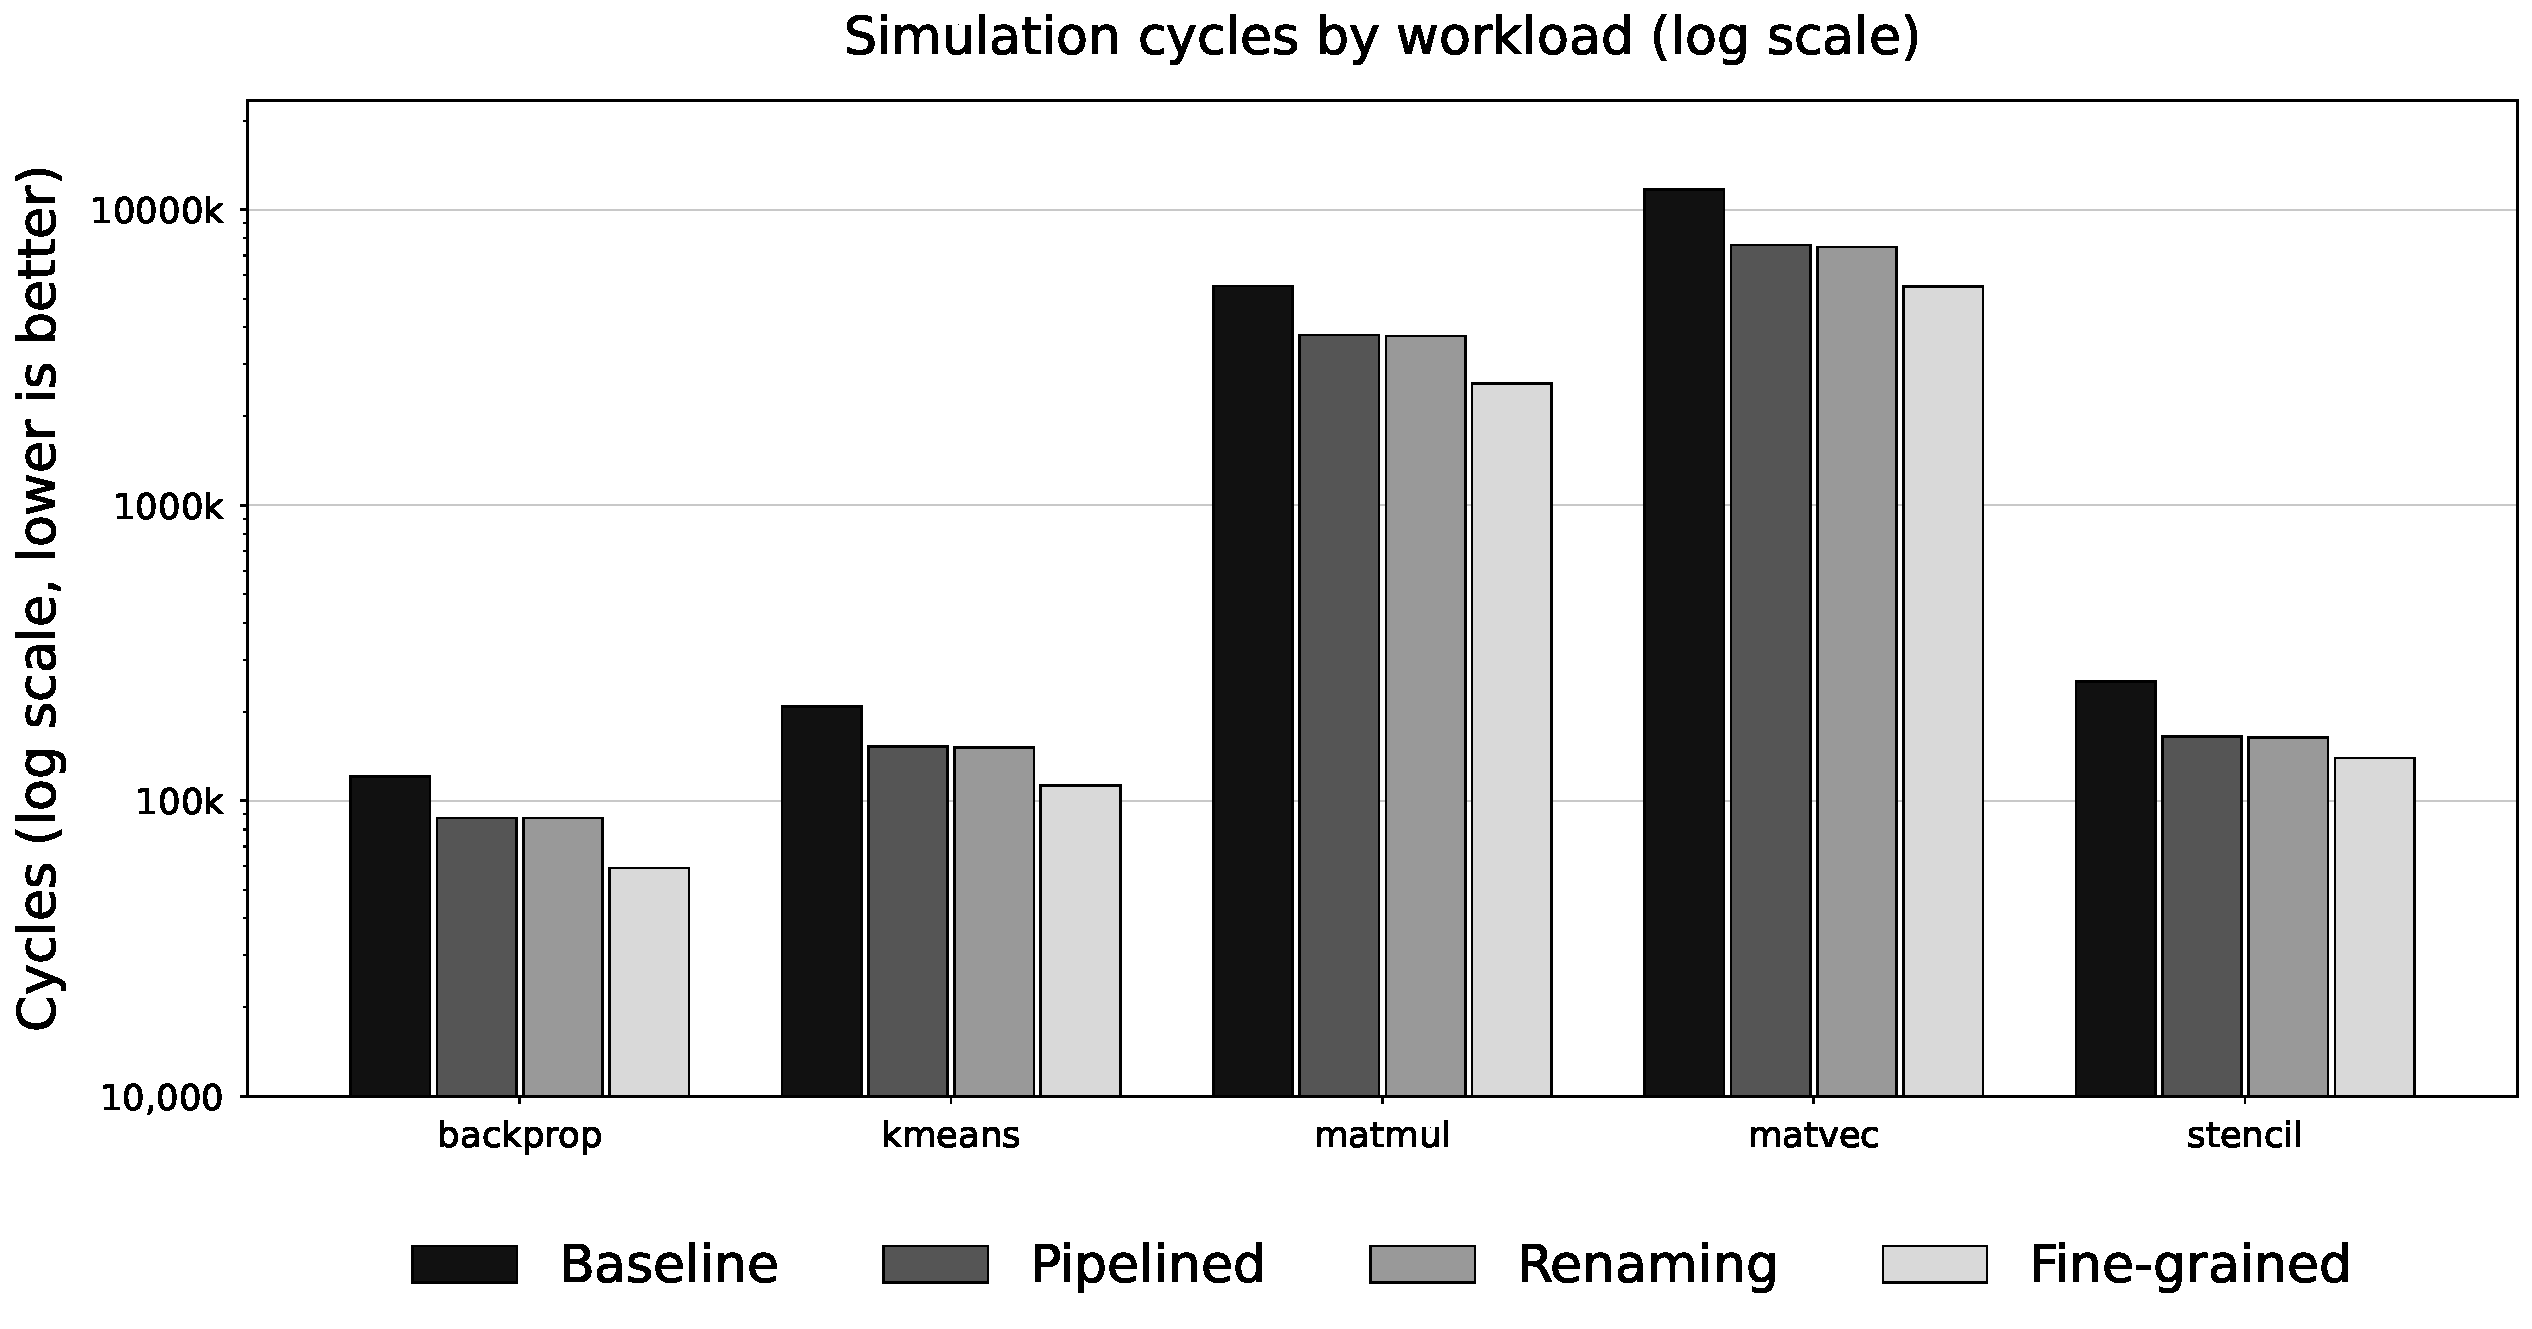
\includegraphics[width=\textwidth]{results/cycles.pdf}
\caption{Total simulated cycles for the five bounded workloads. The logarithmic vertical axis is used to show large and small traces together; cycle counts above 100,000 use the \texttt{k} suffix. Full counts are listed in Table~\ref{tab:timing}.}
\label{fig:cycles}
\end{figure*}

Using the reported speedups rounded to two decimal places, D2 ranges from 1.36$\times$ (K-Means) to 1.54$\times$ (Matvec), and D3 ranges from 1.38$\times$ (K-Means and Backprop) to 1.57$\times$ (Matvec). D4 ranges from 1.81$\times$ (stencil) to 2.14$\times$ (Matmul). Fig.~\ref{fig:speedup} summarizes these speedups. Fig.~\ref{fig:throughput} shows operations per simulated cycle; these values are trace-level simulator metrics, not hardware throughput measurements.

\begin{figure*}[t]
\centering
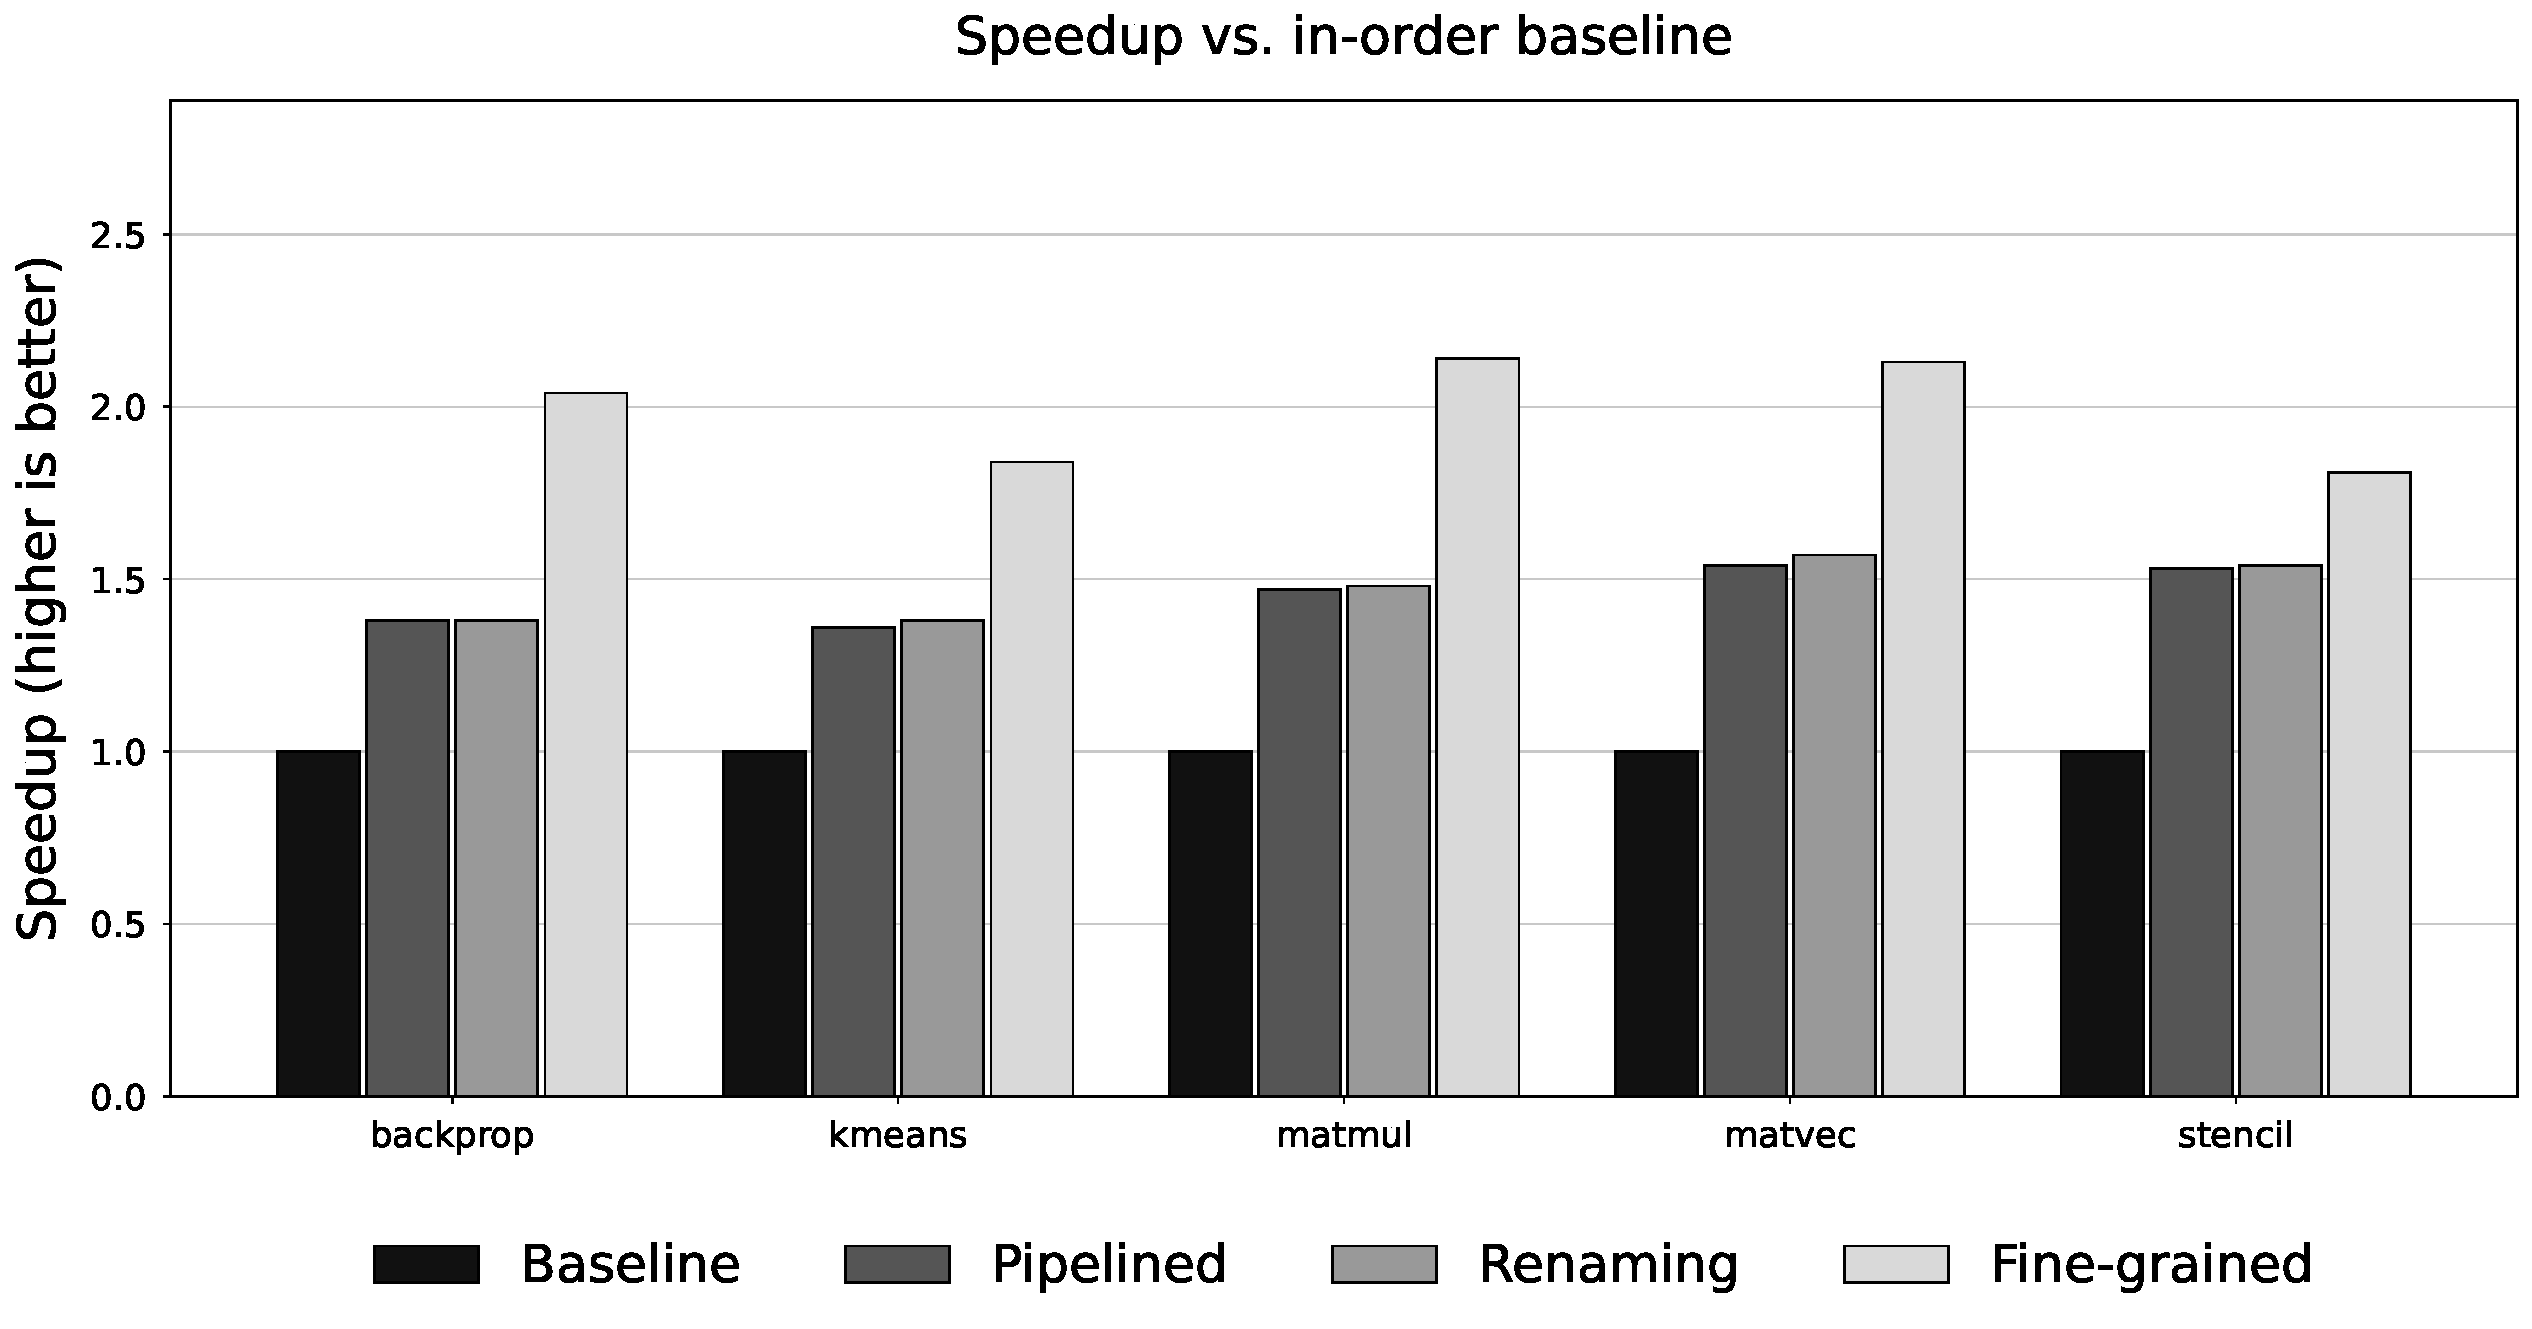
\includegraphics[width=\textwidth]{results/speedup.pdf}
\caption{Speedup relative to D1 for all five workloads, computed from the cycle counts in Table~\ref{tab:timing}.}
\label{fig:speedup}
\end{figure*}

\begin{figure*}[t]
\centering
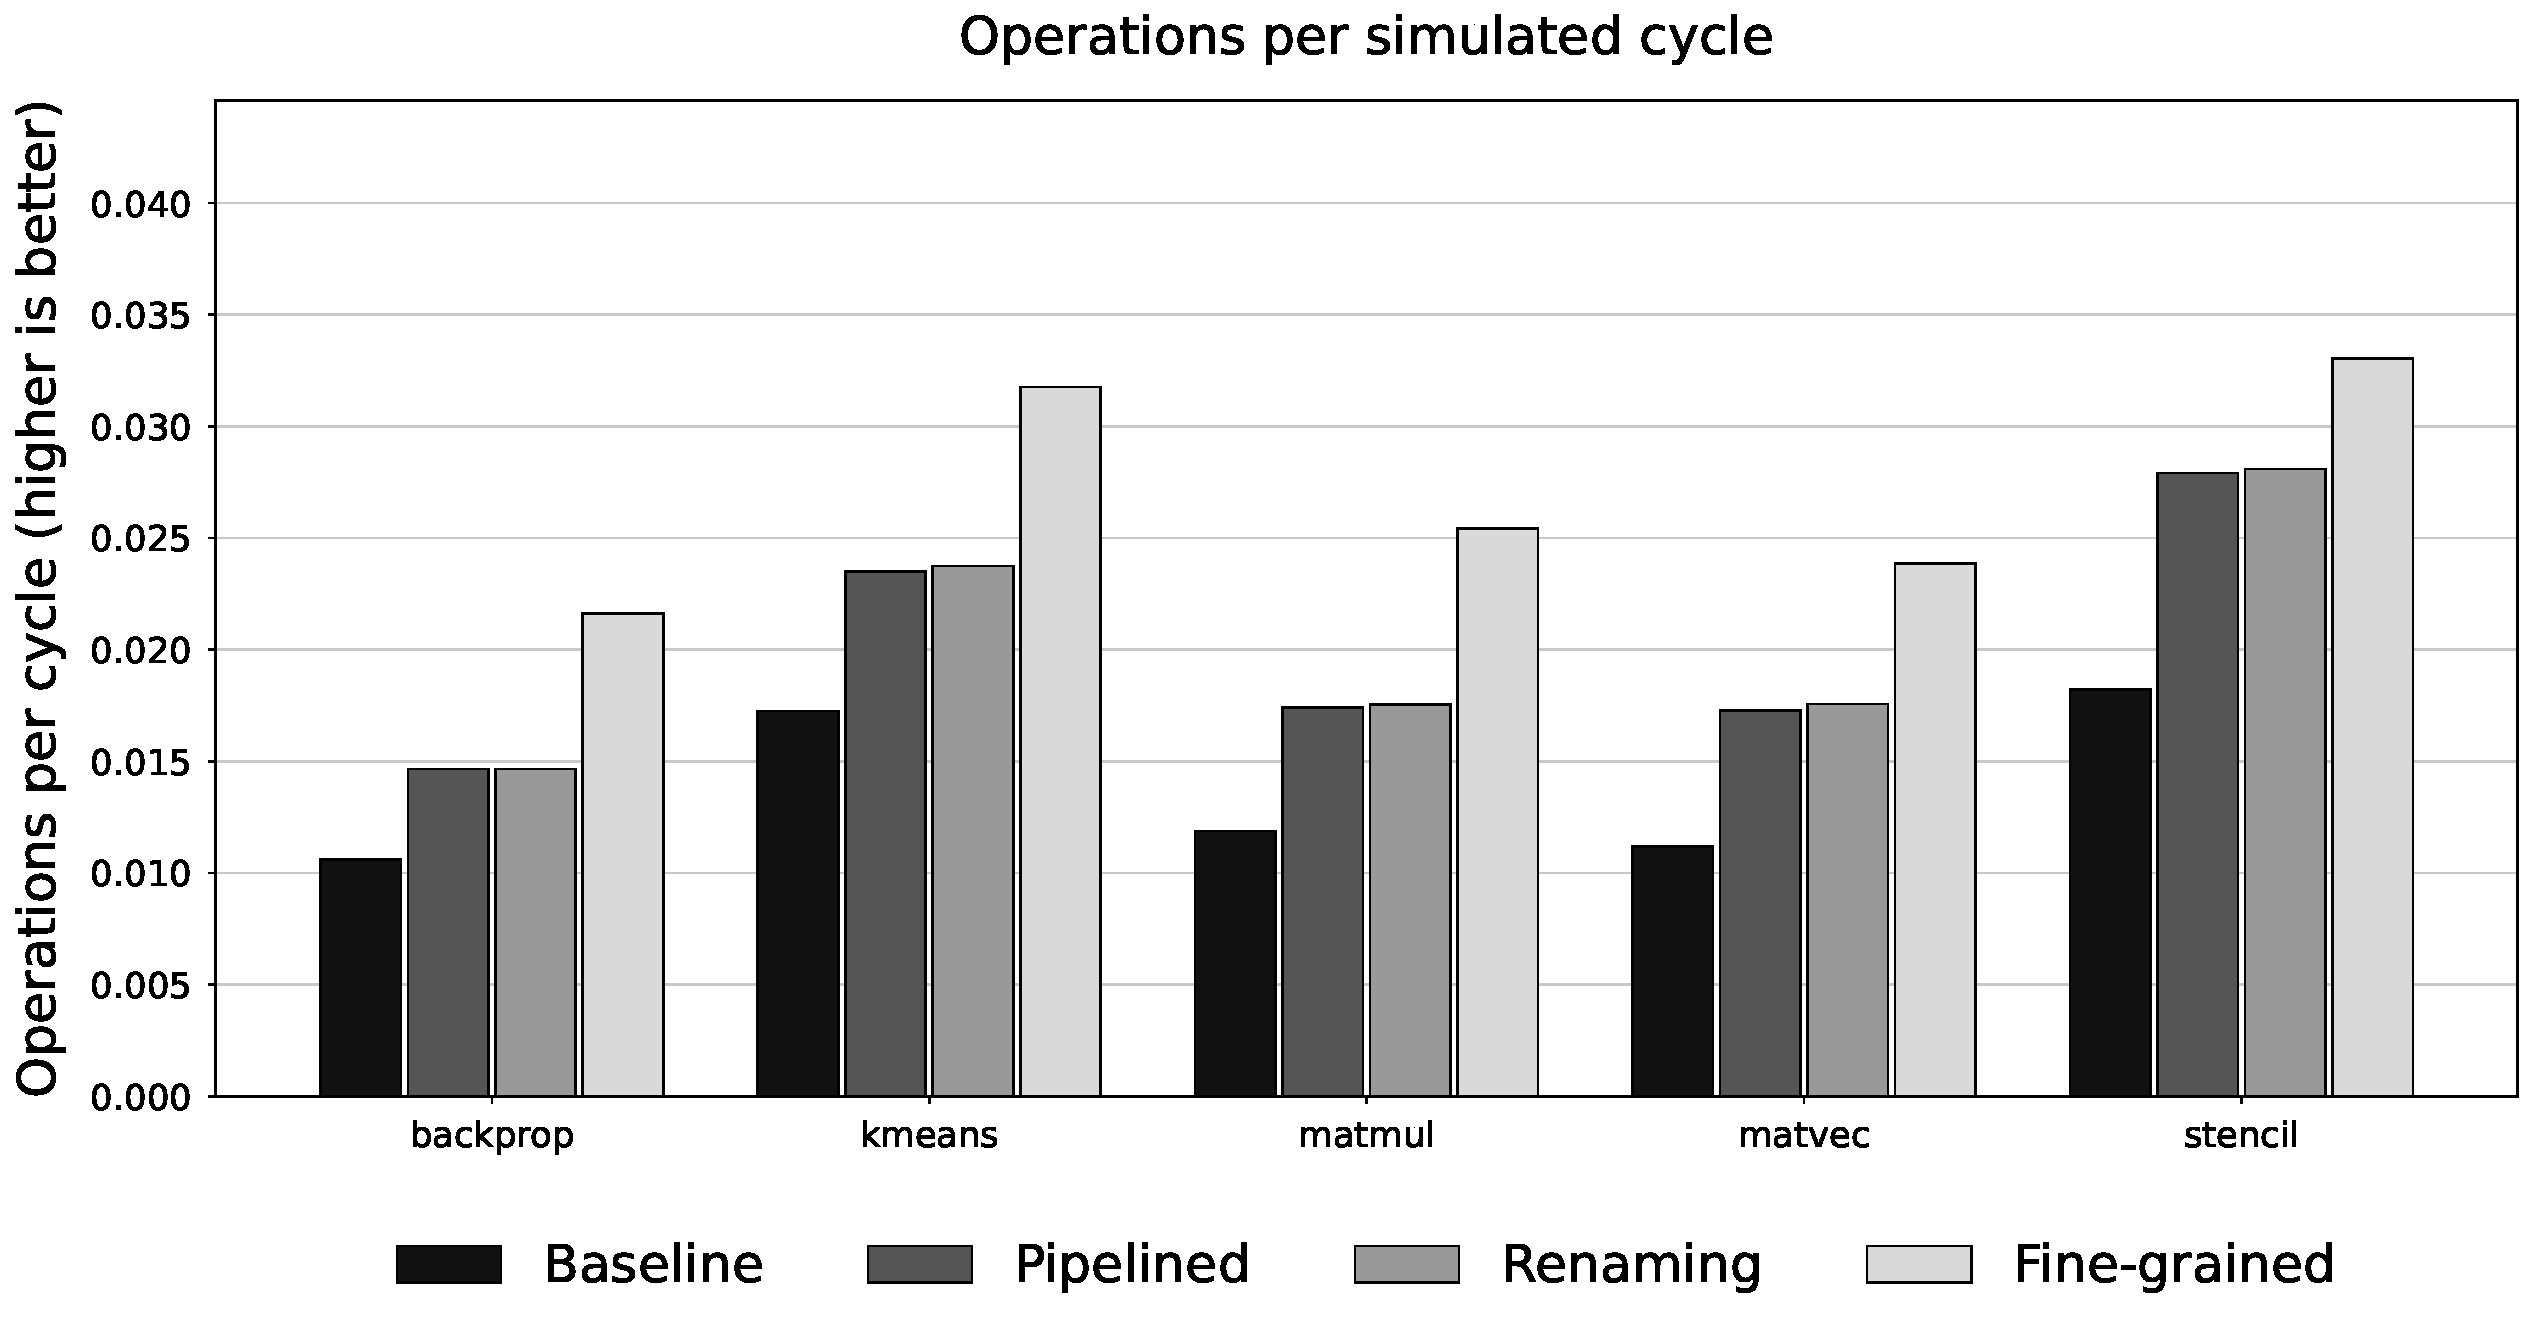
\includegraphics[width=\textwidth]{results/throughput.pdf}
\caption{Trace operations completed per simulated cycle for each design and workload. This derived simulator metric should not be interpreted as measured hardware throughput.}
\label{fig:throughput}
\end{figure*}

All five workloads pass the modeled arithmetic output checks listed in Table~\ref{tab:workloads}. These correctness checks validate the generated trace outputs against their expected values; they do not establish equivalence to complete application benchmark implementations.

\subsection{Measured Host Runtime}
Fig.~\ref{fig:runtime} reports host execution time for the simulator runs. Host time includes simulator and logging overhead and varies with the machine and system load. It is included for reproducibility context and is not used to infer architectural speedup; simulated cycles are the primary comparison metric.

\begin{figure*}[t]
\centering
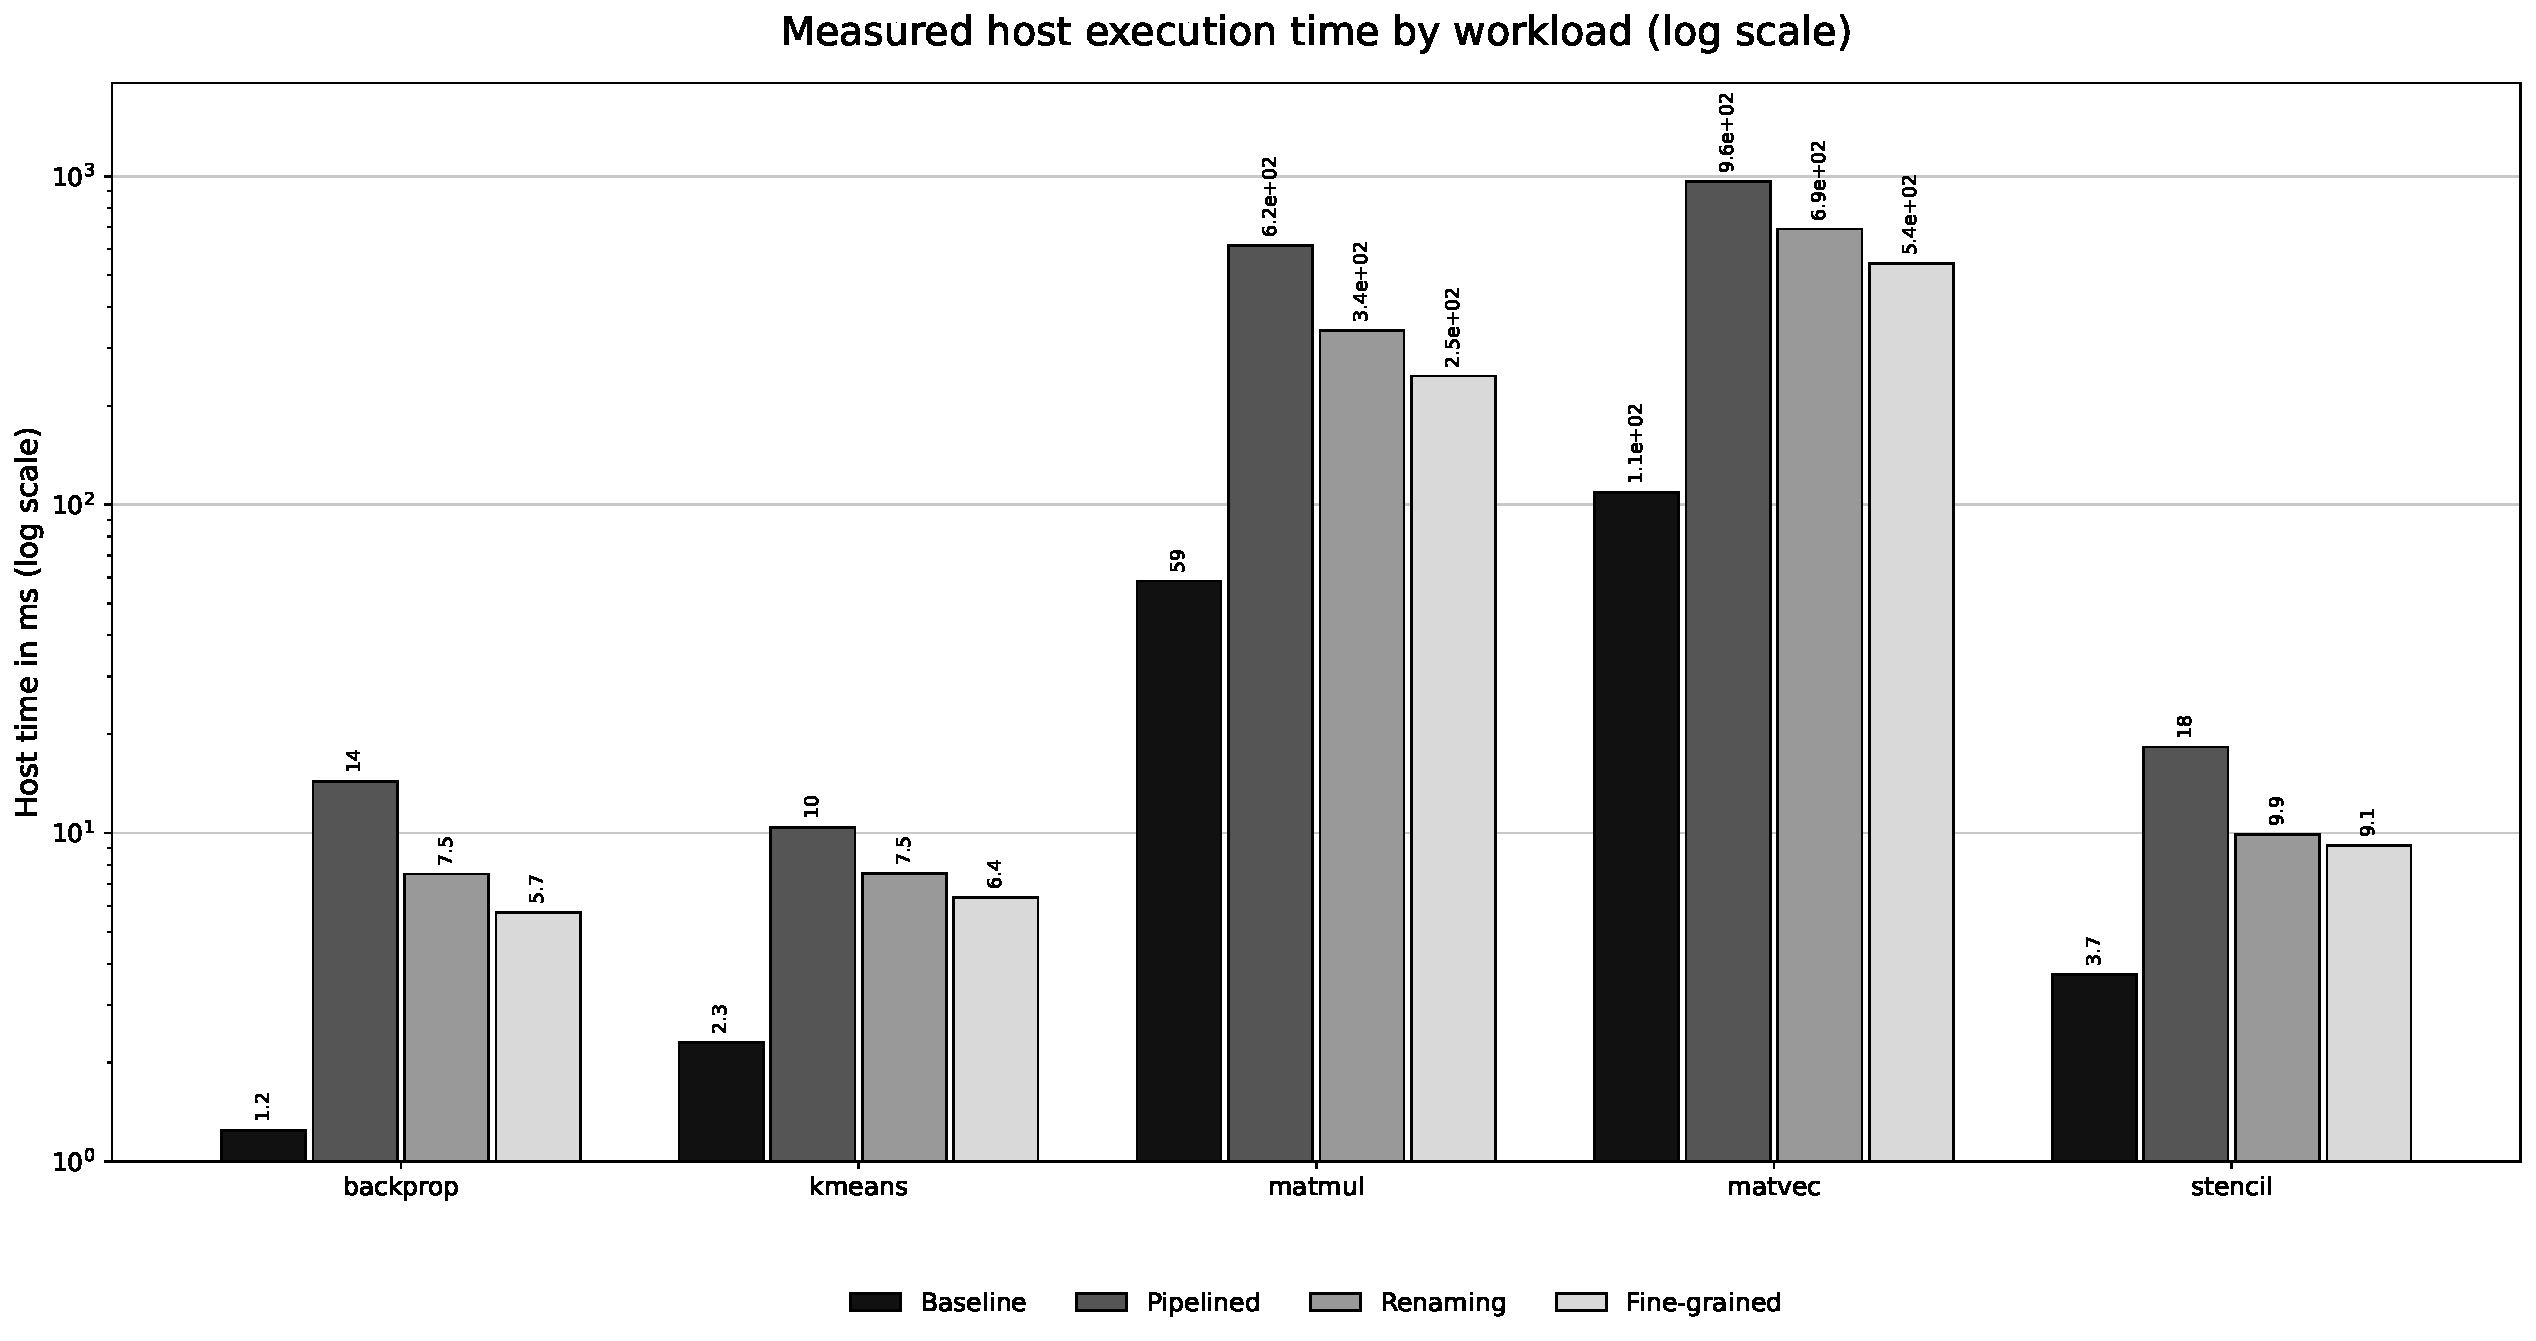
\includegraphics[width=\textwidth]{results/runtime.pdf}
\caption{Host execution time for simulator runs. The logarithmic axis accommodates the workload range; values are machine-dependent and include software and logging overhead.}
\label{fig:runtime}
\end{figure*}


\subsection{Interpretation}
Renaming removes false WAR/WAW dependencies but cannot remove true RAW dependencies or add calculation capacity. Accordingly, the gains from D2 to D3 are modest in these traces, and D3 is slightly slower on Backprop. Fine-grained issue yields larger gains in this model, but its results depend on the modeled memory-visit window, operation latencies, and available independent work. The modeled ranking is not a universal property of the applications or of physical SRAM hardware.


\subsection{Architectural Trade-offs Across Designs}
The four configurations isolate different sources of potential performance improvement. D1 provides a conservative reference in which serialization simplifies control but prevents memory and calculation resources from making progress independently. D2 tests the direct benefit of resource separation: a memory operation and an arithmetic operation can proceed at the same time when they are independent. D3 adds hardware state and bookkeeping for physical-register allocation, source-use tracking, and reclamation. This extra machinery is useful only when false dependencies would otherwise prevent dispatch of independent operations. D4 adds a scheduling opportunity without increasing the number of active memory tasks; it attempts to fill a gap in Port 0 utilization with a calculation that fits within the available visit interval.

These mechanisms have different costs and are not interchangeable. Dual-port pipelining requires the memory and calculation paths to be independently usable. Register renaming requires a sufficiently large physical-register pool and correct reclamation to avoid exhausting free destinations. Fine-grained issue requires the scheduler to know the exact interval in which Port 0 is available and to reject calculations that would conflict with the subsequent writeback. The current simulator abstracts these costs as control and timing rules; it does not quantify area or energy overhead. Consequently, the results should be read as a comparison of modeled scheduling opportunities rather than a complete implementation-cost analysis.

The results also show why workload characterization matters. A workload with independent long-latency arithmetic operations can expose useful overlap between the memory and calculation paths. A workload with frequent control-flow boundaries or true data dependencies may expose fewer independent operations to the dispatcher. Similarly, an operation sequence that does not produce a calculation short enough to fit in the memory-visit window will not benefit from the D4 fallback. This motivates evaluating not only aggregate cycles but also operation mix, dependency distance, branch frequency, memory-phase count, and the fraction of calculations eligible for Port 0 issue.

\section{Limitations and Future Work}
The timing traces are manually generated templates and do not represent complete datasets or full application behavior. The simplified timing model uses one warp, one subarray, one active memory task, and a 16-entry operation table. It does not model bank conflicts, multiple memory channels, cache misses, DRAM traffic, detailed SRAM circuits, area, power, or energy. The Port 0 calculation fallback is a simulator scheduling abstraction and requires validation against a detailed SRAM implementation. The arithmetic checks cover the bounded traces only; they do not establish equivalence to complete application benchmark implementations.

Future work will extend the simulator with multi-bank and multi-subarray behavior, richer traces generated from real kernels, parameter sweeps for table depth and operation latencies, explicit modeling of bank conflicts and memory bandwidth, and power/area-aware evaluation. The operation-table depth and the single-active-memory-task restriction should be varied to determine whether the observed gains persist as concurrency increases. In addition, a trace interface from compiler- or instrumentation-generated programs would reduce dependence on hand-authored operation sequences. A useful validation path is to compare the simulator's phase schedule with a cycle-accurate RTL model and then calibrate the memory-visit and writeback intervals using an SRAM macro model. Finally, energy claims require activity-dependent power estimation; cycle reduction alone is insufficient to infer energy savings. A further step is to validate scheduling decisions against RTL or a circuit-level SRAM model and to investigate compiler support for generating dependency-aware in-SRAM traces.

\section{Conclusion}
This paper presented a language-independent cycle-level simulator for studying four scheduling configurations across five bounded in-SRAM workload traces. Pipelining achieved 1.36$\times$--1.54$\times$ speedup over the in-order baseline, and fine-grained issue achieved 1.81$\times$--2.14$\times$ in the modeled cases. Register renaming provided workload-dependent gains and was slightly slower on Backprop. All arithmetic output checks passed. These results characterize the simulator's assumptions and provide a basis for more detailed architectural modeling; they do not represent full application benchmark executions or measured hardware performance.

\balance
\begin{thebibliography}{00}
\bibitem{aga}
S. Aga, S. Jeloka, A. Subramaniyan, S. Narayanasamy, and D. Blaauw, ``Compute Caches,'' in \textit{Proc. IEEE Int. Symp. High Performance Computer Architecture (HPCA)}, 2017, doi: 10.1109/HPCA.2017.21.

\bibitem{neural}
C. Eckert, X. Wang, J. Wang, A. Subramaniyan, R. R. Iyer, D. Sylvester, D. T. Blaauw, and R. Das, ``Neural Cache: Bit-Serial In-Cache Acceleration of Deep Neural Networks,'' in \textit{Proc. ACM/IEEE Int. Symp. Computer Architecture (ISCA)}, 2018, pp. 383--396, doi: 10.1109/ISCA.2018.00040.

\bibitem{eve}
K. Al-Hawaj, T. Ta, N. Cebry, S. Agwa, O. Afuye, E. Hall, C. Golden, A. B. Apsel, and C. Batten, ``EVE: Ephemeral Vector Engines,'' in \textit{Proc. IEEE Int. Symp. High-Performance Computer Architecture (HPCA)}, 2023, pp. 691--704, doi: 10.1109/HPCA56546.2023.10071074.

\bibitem{duality}
D. Fujiki, S. Mahlke, and R. Das, ``Duality Cache for Data Parallel Acceleration,'' in \textit{Proc. ACM/IEEE Int. Symp. Computer Architecture (ISCA)}, 2019, pp. 397--410, doi: 10.1145/3307650.3322257.

\bibitem{magicache}
R. Fan, Y. Cui, W. Li, M. Wang, and Z. Li, ``MagiCache: A Virtual In-Cache Computing Engine,'' in \textit{Proc. ACM/IEEE Int. Symp. Computer Architecture (ISCA)}, 2025, pp. 1806--1818, doi: 10.1145/3695053.3731113.

\bibitem{repo}
R. Kumari, A. Neogi, P. Nirmalkar, and D. Walia, ``PipeIMC-a-Pipelined-In-SRAM-Computing-Architecture,'' GitHub repository, 2026. [Online]. Available: \url{https://github.com/Ritukrish/PipeIMC-a-Pipelined-In-SRAM-Computing-Architecture}. Accessed: Nov. 9, 2026.

\bibitem{pipeimc}
Y. Cui, R. Fan, W. Li, M. Li, M. Wang, and Z. Li, ``PipeIMC: A Pipelined In-SRAM Computing Architecture,'' in \textit{Proc. ACM/IEEE 53rd Annu. Int. Symp. Computer Architecture (ISCA)}, 2026, pp. 402--415, doi: 10.1109/ISCA66397.2026.00042.
\end{thebibliography}
\end{document}
